\documentclass[10pt]{ctexbeamer}
\usepackage{bm}
\usepackage{tikz}
\usepackage{amsmath}
\usepackage{graphicx}
\newfontfamily{\dengxian}{DengXian}
\newCJKfontfamily{\fzyaoti}{FZYaoTi} %方正姚体
\newCJKfontfamily{\fzjinghong}{FZZJ-JHTJW} %方正字迹-惊鸿体
\newCJKfontfamily{\dqheiti}{Hiragino Sans GB} %冬青黑体
\newCJKfontfamily{\fandolhei}{FandolHei}

% \usetheme[color blocks]{Verona}% 使用Verona主题
% \usetheme[color blocks, red]{Verona}% 使用Verona主题, red theme
% \usetheme[color blocks, gray]{Verona}% 使用Verona主题, grey theme
\usefonttheme[onlymath]{serif}% 数学公式字体设置
\author{Norsesun}
\date{最后更新:\today}
\logo{
\includegraphics[height=1.2cm]{../../../Pngtree owl double exposure.png}}

\definecolor{airforceblue}{rgb}{.36,.54,.66}



\newcommand{\bmc}[1]{$\bm{#1}$}%定义一个新命令,行内数学模式的粗体,使幻灯片上的公式更清楚
\newcommand{\bmcc}[1]{
        \begin{displaymath}
            \bm{#1}
        \end{displaymath}
    }%定义一个新命令,行间数学模式的粗体,使幻灯片上的公式更清楚
\newcommand{\makecenter}[1]{\vspace{0.5em}\centering \parbox{.6\textwidth}{#1}}%定义一个新命令,居中排布一段话
\newenvironment{Mathbreakcenter}[1][1mm]{
        \par
        \vspace{#1} 
        \centering

    }{
        \par
        \vspace{2mm}
    }
\newcommand{\myblock}[3][1-]{
    \centering
    \begin{minipage}{.6\textwidth}
        \begin{block}<#1>{#2}%
            \centering%
            #3
        \end{block}
    \end{minipage}  
    } %定义一个新命令,居中排布一个block

    \newcommand{\myalertblock}[3][1-]{
        \centering
        \begin{minipage}{.6\textwidth}
            \begin{alertblock}<#1>{#2}%
                \centering%
                #3
            \end{alertblock}
        \end{minipage}  
        } %定义一个新命令,居中排布一个alertblock
\newcommand{\cleave}[2]{
    \hbox to #1{} #2 \hbox to #1{}
}
% \newcommand{\annmark}[1]{%
%     \textcolor{red}{$\bm\langle$#1$\bm\rangle$}%
% }%

% \newcommand{\ann}[1]{%
%     \begin{tikzpicture}[remember picture, baseline=-0.75ex]%
%         \node[coordinate] (inText) {};%
%     \end{tikzpicture}%
%     \marginpar{%
%         \renewcommand{\baselinestretch}{1.0}%
%         \begin{tikzpicture}[remember picture]%
%             \definecolor{orange}{rgb}{1,0.5,0}%
%             \draw node[fill=red!20,rounded corners,text width=\marginparwidth] (inNote){\footnotesize#1};%
%     \end{tikzpicture}%
%     }%
%     \begin{tikzpicture}[remember picture, overlay]%
%         \draw[draw = orange, thick]
%             ([yshift=-0.2cm] inText)
%                 -| ([xshift=-0.2cm] inNote.west)
%                 -| (inNote.west);%
%     \end{tikzpicture}%
% }%

% \setlength{\marginparwidth}{2.5cm}
% \renewcommand{\baselinestretch}{1.3}

\newenvironment{mathsalvation}[2][{解:}]{
    \begin{center}{}
        \begin{minipage}[t]{.05\textwidth}
            \vspace{0pt}
            {\color{#2}{#1}} \quad 
        \end{minipage}
        \begin{minipage}[t]{.7\textwidth}
            \vspace{0pt}
            % \fzyaoti
            % \dengxian
            % \fzjinghong
            % \dqheiti
            \fandolhei
}{
    \end{minipage}
    \end{center}
}

\usepackage{smartdiagram}
\usetheme[color blocks, gray]{Verona}% 使用Verona主题, grey theme
\setbeamertemplate{title}[square]


\title{解一元一次方程(2)}
\subtitle{Solve the Equation with one Unknown}

\AtBeginSubsection[\star]
{
	\begin{frame}{要点目录}
		\tableofcontents[currentsubsection]
	\end{frame}
}

\begin{document}
\frame{\titlepage}
    
\section{去括号}
\begin{frame}{去括号}
    \myblock{化简下列各式:}{
        \bmc{(-3a+2b)+3(a-b)}

        \bmc{-5a+4b-(-3a+b)}
    }
\end{frame}

\begin{frame}{温故知新}{去括号的法则}
    \begin{figure}
        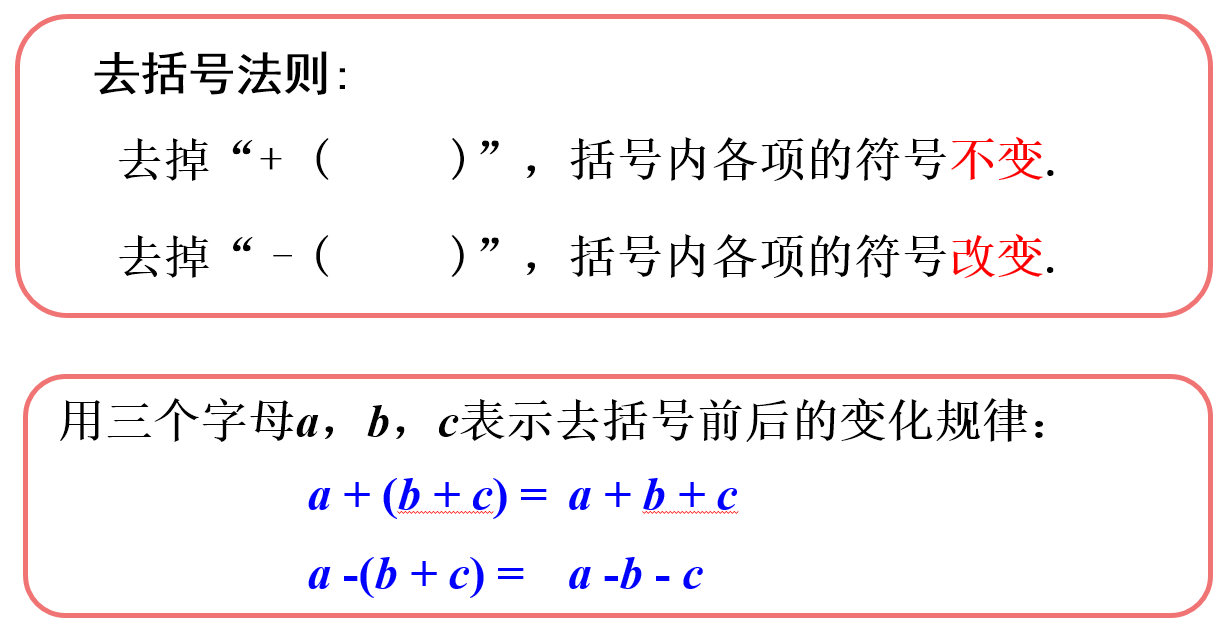
\includegraphics[width=.9\textwidth]{assets/11.png}
    \end{figure}
\end{frame}

\begin{frame}{利用去括号解方程}
    \makecenter{观察下面的方程,结合去括号法则,你能求得它得解吗?}
    \myblock{}{
        \bmc{6x+6(x-2000)=150000}
    }
    \includegraphics<2>[width=.7\textwidth]{assets/12.png}
\end{frame}

\begin{frame}{练习1}
    \myblock{去括号,解方程}{\bmc{3x-7(x-1)=3-2(x+3)}}

    \only<2>{
        \begin{mathsalvation}{red}
            去括号,得
                \begin{Mathbreakcenter}[0.5em]
                    \bmc{3x-7x+7=3-2x-6}
                \end{Mathbreakcenter}
            移项,得
                \begin{Mathbreakcenter}[0.5em]
                    \bmc{3x-7x+2x=3-6-7}
                \end{Mathbreakcenter}
            合并同类项,得
                \begin{Mathbreakcenter}[0.5em]
                    \bmc{-2x=-10}
                \end{Mathbreakcenter}
            系数化为1,得
                \begin{Mathbreakcenter}[0.5em]
                    \bmc{x=5}
                \end{Mathbreakcenter}
        \end{mathsalvation}
    }
\end{frame}
\begin{frame}{解一元一次方程的一般步骤}
    \centering
    \smartdiagram[priority descriptive diagram]{
        {去括号},
        移项,
        合并同类项,
        系数化为1
    }
\end{frame}
\begin{frame}{练习2}
    \myblock{去括号,解方程}{\bmc{7+8(\dfrac{3}{4}x-1)=3x-6(\dfrac{1}{2}-\dfrac{2}{3}x)}}

    \only<2>{
        \begin{mathsalvation}{red}
            去括号,得
                \begin{Mathbreakcenter}[0.5em]
                    \bmc{7+6x-8=3x-3+4x}
                \end{Mathbreakcenter}
            移项,得
                \begin{Mathbreakcenter}[0.5em]
                    \bmc{6x-3x-4x=-3-7+8}
                \end{Mathbreakcenter}
            合并同类项,得
                \begin{Mathbreakcenter}[0.5em]
                    \bmc{-x=-2}
                \end{Mathbreakcenter}
            系数化为1,得
                \begin{Mathbreakcenter}[0.5em]
                    \bmc{x=2}
                \end{Mathbreakcenter}
        \end{mathsalvation}
    }
\end{frame}

\begin{frame}{利用一元一次方程解答实际问题}
    \myblock{}{
        一架飞机在两城之间航行,风速为24 km/h,
        顺风飞行要2小时50分,逆风飞行要3小时,求两城距离。
    }
\end{frame}

\begin{frame}{练习3}
    \myblock{}{
        当\bmc{x}为何值时,式子\bmc{3(x-2)}和\bmc{4(x+3)-4}相等
    }
\end{frame}

\begin{frame}{解有分母的一元一次方程}
    \myblock{}{
        \bmc{\dfrac{3\bm{x}+1}{2}-2=\dfrac{3\bm{x}-2}{10}-\dfrac{2\bm{x}+3}{5}}
    }

    \makecenter{若使方程的系数变成整系数,方程两边应该同乘以什么数?}

    \begin{figure}
        \includegraphics<2>[width=.65\textwidth]{assets/13.png}
    \end{figure}
\end{frame}

\begin{frame}{练习4}
    \myblock{去分母,解方程}{
           \bmc{ \dfrac{\bm{x}-1}{6}- \dfrac{2\bm{x}+1}{3}=1}    
    }
    \only<2>{
    \begin{mathsalvation}{red}
        去分母(方程两边乘6),得
            \begin{Mathbreakcenter}[0.5em]
                \color{red}{
                    \bmc{(x-1)-2(2x+1)=6}
                }
            \end{Mathbreakcenter}
        去括号,得
            \begin{Mathbreakcenter}[0.5em]
                \bmc{x-1-4x-2=6}
            \end{Mathbreakcenter}
        移项,得
            \begin{Mathbreakcenter}[0.5em]
                \bmc{x-4x=6+2+1}
            \end{Mathbreakcenter}
        合并同类项,得
            \begin{Mathbreakcenter}[0.5em]
                \bmc{-3x=9}
            \end{Mathbreakcenter}
        系数化为1,得
            \begin{Mathbreakcenter}[0.5em]
                \bmc{x=-3}
            \end{Mathbreakcenter}
    \end{mathsalvation}}
\end{frame}

\begin{frame}{去分母的总结}
    \begin{enumerate}
        \item 去分母时,应在方程的左右两边乘以分母的\alert{最小公倍数}
        \item 去分母的依据是\alert{等式性质2},去分母时不能漏乘\alert{没有分母的项}
        \item 去分母与去括号这两步分开写,\alert{不要跳步},防止忘记变号
    \end{enumerate}
\end{frame}

\begin{frame}{练习5}
    \myblock{去分母,解方程}{
           \bmc{ \dfrac{4\bm{x}+9}{5}- \dfrac{0.3+0.2\bm{x}}{0.3}=\dfrac{\bm{x}-5}{2}}    
    }

    \only<2>{
    \begin{mathsalvation}{red}
        整理方程,得
            \begin{Mathbreakcenter}[0.3em]
                \color{red}{
                    \bmc{ \dfrac{4\bm{x}+9}{5}- \dfrac{3+2\bm{x}}{3}=\dfrac{\bm{x}-5}{2}}
                }
            \end{Mathbreakcenter}

        去分母(方程两边乘30),得
            \begin{Mathbreakcenter}[0.1em]
                \color{red}{
                    \bmc{6(4x+9)-10(3+2x)=15(x-5)}
                }
            \end{Mathbreakcenter}
        去括号,得
            \begin{Mathbreakcenter}[0.1em]
                \bmc{24x+54-30-20x=15x-75}
            \end{Mathbreakcenter}
        移项,得
            \begin{Mathbreakcenter}[0.1em]
                \bmc{24x-20x-15x=-75-54+30}
            \end{Mathbreakcenter}
        合并同类项,得
                \bmc{-11x=-99}

        系数化为1,得
                \bmc{x=9}
    \end{mathsalvation}}
\end{frame}

\begin{frame}{练习6}
    \begin{block}{}
        \centering
        若代数式\bmc{\dfrac{\bm{x-1}}{2}}与\bmc{\dfrac{6}{5}}
        互为倒数,则\bmc{x=} \uline{\hbox to 20mm{}}?
    \end{block}
\end{frame}

\begin{frame}{练习7}
    \makecenter{
        有一人问老师,他所教的班级有多少学生,
        老师说:“一半学生在学数学,四分之一的学生在学音乐,
        七分之一的学生在学外语,还剩六位学生正在操场踢足球。”
        你知道这个班有多少学生吗? 
    }
\end{frame}
\end{document}